\section{Experimento}
\label{sec:experimento}

Após a obtenção e pré-processamento dos dados, foi realizado o experimento, dividido em seis etapas interligadas, discutidas detalhadamente a seguir.

O conjunto de dados é dividido em treinamento e teste de forma semi-aleatória, onde a frequência de cada classe é respeitada, separando-as proporcionalmente de acordo com a \textbf{Severidade}. Para isso são usados algoritmos de divisão de conjunto de dados do \textit{ScikitLearn} com estratégias de estratificação \cite{sklearn}. O resultado deste processo são dois conjuntos de dados separados, com 80\% dos dados no conjunto de treinamento e os 20\% restantes no conjunto de teste.

\subsection{Etapa de Treinamento}
\label{subsec:etapa-treinamento}

Na etapa de treinamento, os algoritmos de classificação são treinados utilizando o conjunto de treinamento e parâmetros de configuração. Estes parâmetros devem ser ajustados apropriadamente na etapa de otimização, explicada na subseção \ref{subsec:otimizacao}, sendo repetidas estas etapas e as seguintes conforme necessário. O resultado desta etapa são modelos especializados no problema de classificação apresentado pelo conjunto de dados.



\subsection{Etapa de Teste}
\label{subsec:etapa-teste}

A etapa de teste é onde os modelos gerados pelos algoritmos utilizam o conjunto de testes para tentar prever corretamente a classificação de cada caso. O conjunto de estes são os casos restantes após a separação do conjunto de treinamento. A entrada desta etapa é o conjunto de testes e o modelo gerado na etapa de treinamento, enquanto sua saída é uma lista de previsões, corretas ou não.

\section{Métricas de Desempenho}
\label{sec:metricas}

Para comparar os resultados obtidos com os algoritmos de classificação, são utilizadas métricas de desempenho. As predições dos algoritmos são comparadas com os valores reais do conjunto de dados, e a métrica de desempenho é calculada com base nesses valores. As subseções a seguir explicam cada métrica com um exemplo.

\subsection{Matriz de Confusão}
\label{subsec:matriz-confusao}

A matriz de confusão é uma tabela que mostra a quantidade de acertos e erros de cada algoritmo para cada classe \cite{confusion}.

\begin{table}[H] 
  \centering
  \begin{tabular}{l|c|c|}
    \cline{2-3}
    \textbf{}                         & \multicolumn{1}{l|}{\textbf{Predição: LEVE}} & \multicolumn{1}{l|}{\textbf{Predição: GRAVE}} \\ \hline
    \multicolumn{1}{|l|}{\textbf{Real: LEVE}}  & 114631                                       & 85                                            \\ \hline
    \multicolumn{1}{|l|}{\textbf{Real: GRAVE}} & 1949                                         & 4198                                          \\ \hline
  \end{tabular}
  \caption{Exemplo de matriz de confusão binária}
  \label{tbl:tabela-matriz-confusao-metricas} 
\end{table}

O valor na primeira célula, \textbf{Predição: LEVE} e \textbf{Real: LEVE}, indica a quantidade de acertos para a classe LEVE, ou Verdadeiro Positivo (TP), com 114631 acertos. Assim, o valor da segunda célula, \textbf{Predição: GRAVE} e \textbf{Real: LEVE}, indica quantos casos leves foram preditos como graves, chamados de Falsos Positivos (FP), totalizando 85 erros nesta classe.

Da mesma forma, o valor de \textbf{Predição: GRAVE} e \textbf{Real: GRAVE}, indica que houveram 4198 acertos na classe de casos graves, chamados de Verdadeiros Negativos (TN). Igualmente, \textbf{Predição: LEVE} e \textbf{Real: GRAVE} indica quantos casos graves foram preditos como leves, chamados de Falsos Negativos (FN), com 1949 casos graves preditos como leves, uma quantidade considerável e de grande relevância para o problema em questão.

Destes valores, é possível, por meio de cálculos, obter as seguintes métricas.

\begin{table}[H]
  \centering
  \begin{tabular}{c|c|c|c}
    \cline{2-3}
    \textbf{} & \textbf{Positivo Predito} & \textbf{Negativo Predito}         & \textbf{}                              \\ \hline
    \multicolumn{1}{|c|}{\textbf{\begin{tabular}[c]{@{}c@{}}Positivo\\ Predito\end{tabular}}} &
      \begin{tabular}[c]{@{}c@{}}TP\\ 114631\end{tabular} &
      \begin{tabular}[c]{@{}c@{}}FN\\ 85\end{tabular} &
      \multicolumn{1}{c|}{\textit{Sensibilidade}} \\ \hline
    \multicolumn{1}{|c|}{\textbf{\begin{tabular}[c]{@{}c@{}}Negativo\\ Predito\end{tabular}}} &
      \begin{tabular}[c]{@{}c@{}}FP\\ 1949\end{tabular} &
      \begin{tabular}[c]{@{}c@{}}TN\\ 4198\end{tabular} &
      \multicolumn{1}{c|}{\textit{Especificidade}} \\ \hline
    \textbf{} & \textit{Precisão}         & \textit{Valor Preditivo Negativo} & \multicolumn{1}{c|}{\textit{Acurácia}} \\ \cline{2-4} 
  \end{tabular}
  \caption{Exemplo de métricas de uma matriz de confusão binária}
  \label{tbl:tabela-matriz-confusao-metricas-explicado}  
\end{table}

\subsection{Acurácia}
\label{subsec:acuracia}

A acurácia indica a quantidade de casos que foram preditos corretamente.

  \begin{equation}
    \textbf{Acurácia} = \frac{TP + TN}{TP + TN + FP + FN}
  \end{equation}

Portanto, a execução do \textit{Random Forest} de exemplo, com a matriz de confusão acima, obteve uma acurácia de 0,98317, ou 98,317\%.

\subsection{Precisão}
\label{subsec:precisao}

A precisão indica a quantidade de casos leves que foram preditos corretamente, dividido pelo total de predições positivas. Essa métrica serve para o julgamento da veracidade dos casos leves preditos, porém ignora os casos graves.

  \begin{equation}
    \textbf{Precisão} = \frac{TP}{TP + FP}
  \end{equation}

Assim, a execução de exemplo obteve uma precisão de 98,328\%.

\subsection{Valor Preditivo Negativo}
\label{subsec:valor-preditivo-negativo}

A precisão também pode ser chamada de valor preditivo positivo, então o valor preditivo negativo é a precisão dos casos negativos, ou casos graves, indicando a quantidade de casos graves que foram preditos corretamente, divido pelo total de predições negativas. Da mesma forma, a métrica ignora os casos leves, mas traz confiança que os casos graves são realmente graves.

  \begin{equation}
    \textbf{Valor Preditivo Negativo} = \frac{TN}{TN + FN}
  \end{equation}

A execução de exemplo obteve um valor preditivo negativo de 98,015\%

\subsection{Precisão Macro}
\label{subsec:precisao-macro}

É possível utilizar a precisão de cada classe para calcular a precisão macro. Em conjuntos com apenas duas classes, a precisão macro é a média da precisão e do valor preditivo negativo, sendo mais dinâmica.

  \begin{equation}
    \textbf{Precisão Macro} = \frac{1}{N}\sum_{i=1}^{N}\frac{TP_{i}}{TP_{i} + FP_{i}}
  \end{equation}

A média das métricas então resulta em 98,171\%.


\subsection{Sensibilidade}
\label{subsec:sensibilidade}

\textit{Recall}, ou sensibilidade, indica a quantidade de casos leves que foram preditos corretamente, dividido pelo total de casos leves. A sensibilidade então serve como uma medida de que as predições não vão resultar em alarmes falsos, prevendo casos leves como graves.

  \begin{equation}
    \textbf{Sensibilidade} = \frac{TP}{TP + FN}
  \end{equation}

Obtendo um valor de 99,925\%, com uma baixa quantidade de falsos negativos.

\subsection{Especificidade}
\label{subsec:especificidade}

A especificidade indica a quantidade de casos graves que foram preditos corretamente, dividido pelo total de casos graves. É equivalente à sensibilidade dos casos graves, medindo os casos graves que foram julgados como LEVE, com grande relevância para o conjunto de dados em questão.

  \begin{equation}
    \textbf{Especificidade} = \frac{TN}{TN + FP}
  \end{equation}

Obtendo um valor de 68,293\%, relativamente baixa confiança em casos graves, significando que mais de 30\% dos casos graves não foram classificados corretamente.

\subsection{Sensibilidade Macro}
\label{subsec:sensibilidade-macro}

Similar à precisão macro, a sensibilidade macro é a média da sensibilidade e da especificidade em conjuntos de dados binários, medindo os falsos positivos e falsos negativos.

  \begin{equation}
    \textbf{Sensibilidade Macro} = \frac{1}{N}\sum_{i=1}^{N}\frac{TP_{i}}{TP_{i} + FN_{i}}
  \end{equation}

A média então resulta em 84,109\%, que, em comparação com a sensibilidade, informa que a especificidade está baixa.

\subsection{F1-Score}
\label{subsec:f1-score}

O \textit{F1-Score}, ou F1, é uma métrica composta que utiliza a média harmônica da precisão e da sensibilidade, de forma a medir tanto predições corretas quanto predições falsas dos casos leves.

\begin{equation}
  \textbf{F1-Score} = 2\times\frac{Precis.\times Sensib.}{Precis. + Sensib}
\end{equation}

Alternativamente:
\begin{equation}
  \textbf{F1-Score} = \frac{2TP}{2TP + FP + FN}
\end{equation}

Assim obtendo um valor de 99,120\%, um valor alto, demonstrando que as predições de casos leves são confiáveis.
A mesma métrica pode ser aplicada à classe de casos graves, resultando em 80,5\%, um valor bem mais baixo em comparação.

\subsection{F1-Score Macro}
\label{subsec:f1-score-macro}

É possível então utilizar o \textit{F1-score} de cada classe para calcular o \textit{F1-score} macro, levando em conta não só a precisão e a sensibilidade, mas também o valor preditivo negativo e a especificidade, sendo uma média entre os \textit{F1-scores} das classes.

  \begin{equation}
    \textbf{F1-Score Macro} = \frac{1}{N}\sum_{i=1}^{N}\frac{2TP_{i}}{2TP_{i} + FP_{i} + FN_{i}}
  \end{equation}

Obtendo-se assim um valor que considera todas as métricas anteriores, 89,810\%, trazendo uma visão mais ampla do desempenho do algoritmo em questão.

\subsection{AUC ROC}
\label{subsec:curva-roc}

Além do \textit{F1-score}, é possível utilizar as métricas calculadas para plotar a curva Característica de Operação do Receptor (ROC), tendo a sensibilidade no eixo Y contra a especificidade invertida no eixo X. A curva permite não só visualizar o desempenho do classificador e encontrar o ponto ótimo da sensibilidade em função da especificidade, sendo o ponto mais próximo da esquerda superior \cite{roc}.

\begin{figure}[ht!]
  \centering
  \fcolorbox{white}{white}{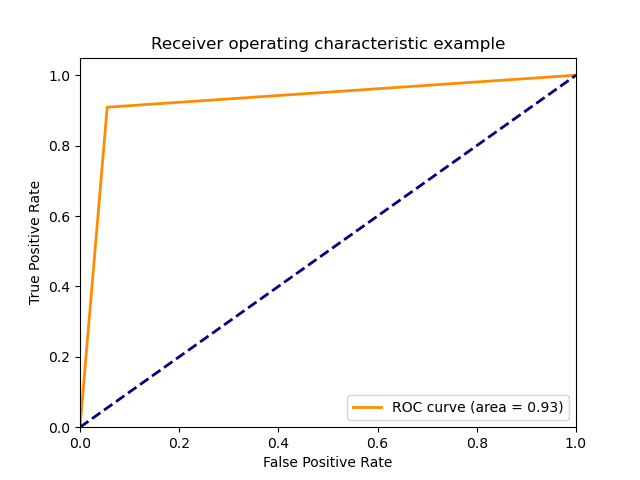
\includegraphics[width=0.5\textwidth]{chapters/metodologia/images/roc.png}}
  \caption{\textmd{Curva ROC de uma execução de XGBoost}}
  \label{fig:curva-roc-exemplo}
\end{figure}

Com a curva, é possível então calcular a Área Abaixo da Curva (AUC), onde um modelo com 0\% de acurácia teria um AUC de 0, e um modelo com 100\% de acurácia teria um AUC de 1. Na figura \ref{fig:curva-roc-exemplo}, o modelo de exemplo alcançou um AUC de 93,768\%.

\subsection{Otimização de Parâmetros}
\label{subsec:otimizacao}

A etapa de otimização de parâmetros consiste em ajustar os parâmetros de configuração dos algoritmos de classificação para que sejam o mais adequados o possível aos dados de treinamento. Para avaliar isso, são usadas as métricas obtidas na etapa anterior. De acordo com a necessidade, as etapas anteriores são executadas múltiplas vezes de modo a obter o melhor resultado.

Para facilitar esse processo, foi utilizada a técnica de otimização de parâmetros (\textit{grid search}) do \textit{ScikitLearn} \cite{sklearn}. O \textit{grid search} tenta encontrar os melhores parâmetros de forma automatizada, executando uma busca exaustiva com diversos parâmetros de cada algoritmo \cite{gridsearch}.

Notou-se que o conjunto de dados estava desbalanceado, ou seja, a quantidade de casos leves era 20 vezes maior que a quantidade de casos graves. Portanto, se viu necessário aplicar a técnica de balanceamento de conjunto de dados \textit{RandomUnderSampler}. Os registros da classe mais comum são removidos aleatoriamente para balancear as classes. Então a quantidade casos leves e torna igual à de casos graves no conjunto de dados balanceado.

\subsection{Geração de Gráficos}
\label{subsec:geracao-graficos}

Tendo um modelo do algoritmo de classificação satisfatório, foram gerados então diversos gráficos interpretáveis para a análise dos dados. Em especial os gráficos SHAP para entender a interpretação do modelo sobre o conjunto de dados na importância de cada variável \cite{shap}. 

\begin{figure}[ht!]
  \centering
  \fcolorbox{white}{white}{\includegraphics[width=0.5\textwidth]{chapters/resultados/images/xgboost_normal_dot.png}}
  \caption{\textmd{Gráfico SHAP de interpretação de relevância de atributos.}}
  \legend{Fonte: \textit{SHAP documentation}}
  \label{fig:shap-exemplo}
\end{figure}

Gráficos SHAP de pontos como na figura \ref{fig:shap-exemplo} de exemplo combinam gráficos de dispersão com estimativas de densidade. A cor dos pontos significa o valor do atributo, onde pontos azuis significam que o valor do atributo é baixo ou falso, enquanto pontos vermelhos significam que o valor é alto ou verdadeiro. A posição horizontal dos pontos representa o impacto do atributo no resultado da classificação, onde pontos na esquerda significam que aquele valor é importante na classificação negativa, e pontos na direita na classificação positiva.


Também é possível gerar gráficos de análise do conjunto de dados, como gráficos de Mapas de Calor de Correlação \cite{correlation} e Plotagens de Densidade das Colunas \cite{density}, que também podem servir como fonte de informação para a análise dos dados.

\subsection{Subconjuntos}
\label{subsec:subconjuntos}

Foi observado que o conjunto de dados permite diferentes cenários por meio de subconjuntos, podendo oferecer \textit{insights} sobre os resultados, fatores de risco e impactos das variáveis. Portanto, as seguintes análises são propostas.

\subsubsection{Omitir dados sintomáticos}
\label{subsubsec:omitindosintomas}

O conjunto de dados utilizado no experimento possui 20 colunas de dados sintomáticos apresentados pelos pacientes após confirmado o diagnóstico de COVID-19. Ao omitir essas colunas, é possível observar como os algoritmos predizem os casos leves e graves se baseando somente nos dados demográficos, doenças preexistentes e progresso da vacinação. Idealmente, será possível perceber fatores de risco demográficos e clínicos antes mesmo do paciente contrair COVID-19, permitindo uma melhor priorização de tratamento.

\subsubsection{Possibilidade de óbito}
\label{subsubsec:analisandoobito}

Cerca de 1/4 dos casos graves resultaram em óbito do paciente, como demonstrado na coluna \textbf{Data de Óbito}. Por meio desta, é possível comparar casos onde não houve óbito com casos que resultaram em óbito, em um conjunto de dados binário. Sendo assim, é possível identificar especificamente fatores de risco que podem ocasionar no óbito do paciente.

\subsubsection{Progresso da vacinação}
\label{subsubsec:progressovacinacao}

Filtrando o conjunto de dados pelas colunas de vacinação, é possível identificar mudanças nos fatores de risco, de modo a perceber os impactos da vacinação no Recife de acordo com seu progresso. Se propõe então observar a situação antes do início da vacinação, assim como depois de um certo progresso da vacinação, para identificar possíveis impactos. 


